%===============================================================
% CHAPTER 2 – Comparative Matrix with Weighted Average Calculations
%===============================================================
\chapter{Comparative Matrix with Weighted Average Calculations}
\label{chap:matrix}

\section{Candidate Concept Definitions}

Four candidate UAV configurations were considered for evaluation. Each option represents a different balance of manufacturing complexity, aerodynamic efficiency, and mission suitability:

\begin{description}[noitemsep]
    \item[Option A] \textbf{Standard quadrotor with roof-mounted solar array.}   

    
    This is the most conventional design, relying on four fixed rotors for lift and stability. The solar array is mounted flat on the upper surface of the frame to provide supplemental energy. Its advantages include simplicity of construction, mature control algorithms, and high feasibility for student prototyping. However, it suffers from poor cruise efficiency, limited range, and continuous high power draw during hover.

    \item[Option B] \textbf{Dual-axis tilt-rotor (wing-tip motors only, no rear motor).}  


    
    This configuration places two tilt-rotor nacelles at the wing tips, allowing transition between vertical and forward flight. It reduces structural weight compared to three-axis designs but introduces challenges in stability and redundancy. Without a rear motor, yaw control and payload balance are more demanding. Manufacturing complexity is moderate, but the design offers a useful compromise between efficiency and mechanical simplicity.

    \item[Option C] \textbf{Three-axis tilt-rotor + rear pusher (Solift -- selected configuration).}  

    
    The Solift concept integrates two wing-tip tilt rotors with a rear pusher motor, enabling efficient cruise while maintaining vertical take-off and landing capability. This design maximizes functional relevance for logistics missions, as it combines hover stability, efficient wing-borne flight, and redundancy in propulsion. It is mechanically more complex, requiring precise tolerances in tilt mechanisms, but it provides the richest ground for Design for Manufacturing analysis and innovation potential.

    \item[Option D] \textbf{Pure fixed-wing with ETFE solar skin and catapult launch.}  

    
    This option prioritizes aerodynamic efficiency and solar harvesting by covering a large wing area with ETFE-encapsulated photovoltaic cells. It achieves excellent lift-to-drag ratios and extended range under daylight conditions. However, it lacks VTOL capability, requiring external launch and recovery systems such as catapults or runways. While attractive for endurance missions, it is less suited to urban logistics scenarios where compact landing and take-off are essential.
\end{description}


\section{Evaluation Criteria and Weight Assignment}

The evaluation criteria were defined based on the mission profile (urban logistics, 10--30~km radius, 5~kg payload) and DFM considerations. The weight assignments are shown in Table~\ref{tab:weights}.

\begin{table}[H]
\centering
\caption{Evaluation Criteria and Weight Assignment}
\label{tab:weights}
\begin{tabularx}{\textwidth}{C{0.5cm} L{5cm} C{2cm} L{5cm}}
\toprule
\textbf{\#} & \textbf{Criterion} & \textbf{Weight (\%)} & \textbf{Rationale} \\
\midrule
1 & Manufacturing complexity & 20 & Must be challenging enough for DFM analysis but feasible for students \\
2 & Data availability & 15 & Requires measurable/testable parameters (solar, wing, CAD) \\
3 & Feasibility & 20 & Must be prototypable with accessible materials and tools \\
4 & Functional relevance & 20 & Should address logistics delivery and VTOL needs \\
5 & Innovation potential & 15 & Should combine technologies in a novel way \\
6 & DFM learning value & 10 & Must reveal trade-offs in design vs. manufacturing \\
\midrule
& \textbf{Total} & \textbf{100} & \\
\bottomrule
\end{tabularx}
\end{table}

\section{Scoring Scale Definition}

All options are scored on a \textbf{1--10 integer scale} per criterion, where:

\begin{itemize}[noitemsep]
    \item \textbf{10} -- Excellent: fully meets or exceeds requirement
    \item \textbf{7--9} -- Good: meets requirement with manageable trade-offs
    \item \textbf{4--6} -- Acceptable: partially meets requirement; notable weaknesses
    \item \textbf{1--3} -- Poor: fails to meet requirement or introduces major risk
\end{itemize}

\section{Comparative Matrix and Scoring}

Table~\ref{tab:matrix_raw} presents the raw scores assigned to each option per criterion.

\begin{table}[H]
\centering
\caption{Raw Score Comparative Matrix (Scale 1--10)}
\label{tab:matrix_raw}
\begin{tabularx}{\textwidth}{L{4.5cm} C{1.8cm} C{1.8cm} C{1.8cm} C{1.8cm} C{1.8cm}}
\toprule
\textbf{Criterion} & \textbf{Weight} & \textbf{Option A} & \textbf{Option B} & \textbf{Option C} & \textbf{Option D} \\
\midrule
Manufacturing complexity & 0.20 & 5 & 7 & 9 & 6 \\
Data availability & 0.15 & 6 & 6 & 9 & 7 \\
Feasibility & 0.20 & 9 & 7 & 8 & 6 \\
Functional relevance & 0.20 & 5 & 7 & 9 & 6 \\
Innovation potential & 0.15 & 4 & 6 & 9 & 7 \\
DFM learning value & 0.10 & 5 & 7 & 9 & 6 \\
\bottomrule
\end{tabularx}
\end{table}

Figure~\ref{fig:matrix-sketch} shows the original hand-drawn scoring sheet produced during the initial design review session, from which the values in Table~\ref{tab:matrix_raw} were formalised.

\begin{figure}[htbp]
    \centering
    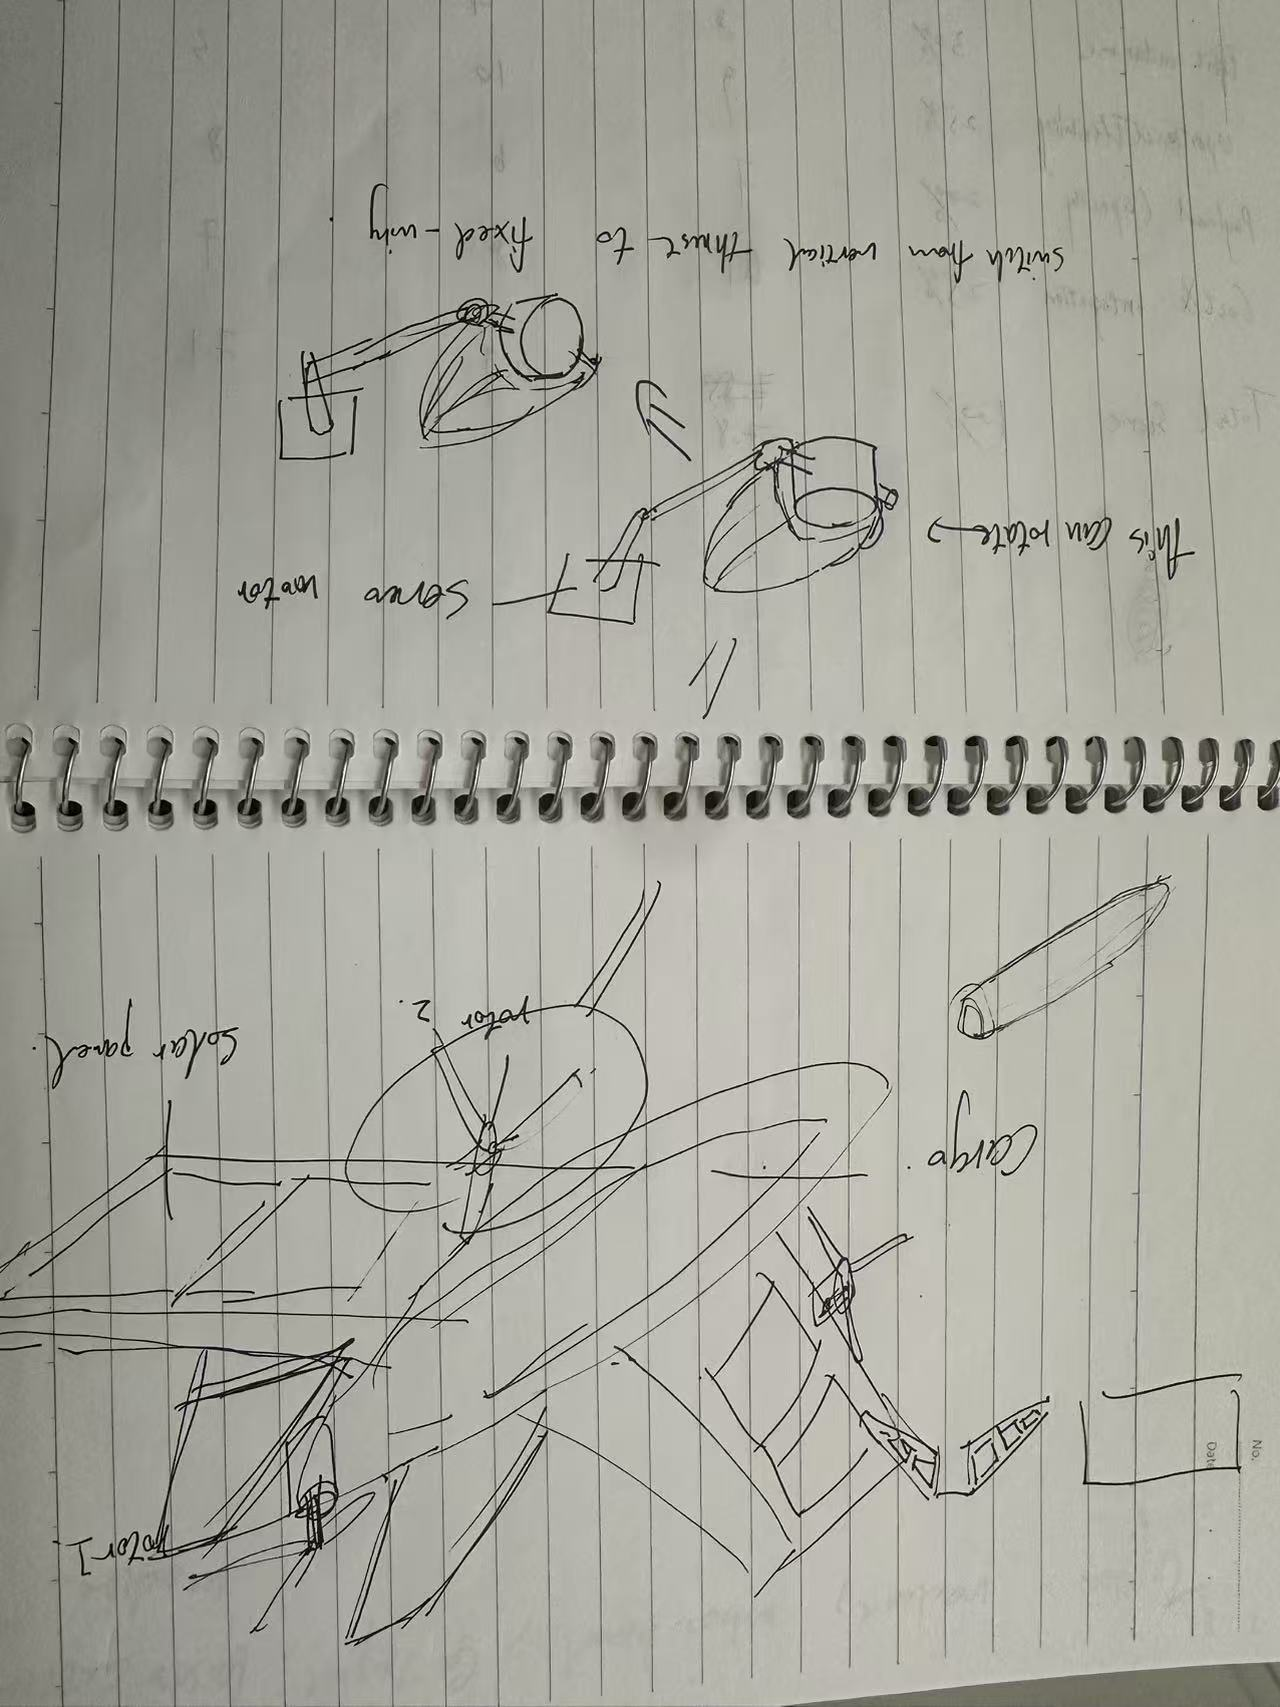
\includegraphics[width=0.82\textwidth]{figures/Solift_schematic.jpg}
    \caption{Hand-drawn comparative matrix scoring sheet from the initial design review.}
    \label{fig:matrix-sketch}
\end{figure}

\section{Weighted Average Calculations (Step-by-Step)}

The weighted score for each option is computed as:
\begin{equation}
    S_{option} = \sum_{i=1}^{n} w_i \cdot s_i
    \label{eq:weighted}
\end{equation}

\subsection{Option A -- Quadrotor}


\[
S_A = (0.20 \times 5) + (0.15 \times 6) + (0.20 \times 9) + (0.20 \times 5) + (0.15 \times 4) + (0.10 \times 5) = \mathbf{6.0}
\]



\subsection{Option B -- Dual Tilt}


\[
S_B = (0.20 \times 7) + (0.15 \times 6) + (0.20 \times 7) + (0.20 \times 7) + (0.15 \times 6) + (0.10 \times 7) = \mathbf{6.7}
\]



\subsection{Option C -- Solift}


\[
S_C = (0.20 \times 9) + (0.15 \times 9) + (0.20 \times 8) + (0.20 \times 9) + (0.15 \times 9) + (0.10 \times 9) = \mathbf{8.8}
\]



\subsection{Option D -- Fixed Wing}


\[
S_D = (0.20 \times 6) + (0.15 \times 7) + (0.20 \times 6) + (0.20 \times 6) + (0.15 \times 7) + (0.10 \times 6) = \mathbf{6.4}
\]



\section{Final Ranking and Selection Justification}

\begin{table}[H]
\centering
\caption{Final Weighted Scores and Ranking}
\label{tab:matrix_final}
\begin{tabularx}{\textwidth}{C{0.5cm} L{5cm} C{3cm} C{2.5cm} L{3cm}}
\toprule
\textbf{Rank} & \textbf{Option} & \textbf{Weighted Score} & \textbf{Normalised (\%)} & \textbf{Verdict} \\
\midrule
1 & \textbf{Option C -- Solift (3-axis)} & \textbf{8.8} & \textbf{100\%} & \textbf{Selected} \\
2 & Option B -- Dual Tilt & 6.7 & 76\% & Rejected (less redundancy) \\
3 & Option D -- Fixed Wing & 6.4 & 73\% & Rejected (no VTOL capability) \\
4 & Option A -- Quadrotor & 6.0 & 68\% & Rejected (limited cruise efficiency) \\
\bottomrule
\end{tabularx}
\end{table}

\noindent \textbf{Conclusion:} Option C (Solift) achieves the highest weighted score and is confirmed as the selected design. It balances manufacturing complexity, functional relevance, and innovation potential, while being supported by real test data and CAD models.
